\documentclass[final,1p,times,authoryear]{elsarticle}
\usepackage{amsmath}
\usepackage{amsthm}
\usepackage{amssymb}
\usepackage{amsfonts}

\newtheorem{theorem}{Theorem}
\newtheorem{lemma}[theorem]{Lemma}
\newtheorem{corollary}[theorem]{Corollary}
\newtheorem{conjecture}[theorem]{Conjecture}
\newtheorem{proposition}[theorem]{Proposition}
\newtheorem{definition}[theorem]{Definition}
\newtheorem{notation}[theorem]{Notation}
\newtheorem{example}[theorem]{Example}
\newtheorem{remark}[theorem]{Remark}
\newtheorem{problem}[theorem]{Problem}
\newtheorem{acknowledgment}[]{Acknowledgment}
\iffalse
\newenvironment{proof}{\noindent{\em Proof:}}{$\Box$~\\}
\fi


\usepackage{comment}
\usepackage{url}
\usepackage{tikz}
\usepackage{graphicx}
\usepackage{gclc}

\def\d{{\fontencoding{T1}\selectfont\dj}}
\def\D{{\fontencoding{T1}\selectfont\DJ}}

%za sirinu tabele
\usepackage{array}
\newcolumntype{L}[1]{>{\raggedright\let\newline\\\arraybackslash\hspace{0pt}}m{#1}}
\newcolumntype{C}[1]{>{\centering\let\newline\\\arraybackslash\hspace{0pt}}m{#1}}
\newcolumntype{R}[1]{>{\raggedleft\let\newline\\\arraybackslash\hspace{0pt}}m{#1}}


\begin{document}

\begin{frontmatter}

\title{Integrating algebraic theorem provers with dynamic geometry
  systems for solid geometry\footnote{This work was partially
    supported by the Serbian Ministry of Science grant 174021}}

\author{Danijela Simi\' c}
\address{School of Mathematics, University of Belgrade, Studentski trg 16, 11000, Belgrade, Serbia}
\ead{danijela@matf.bg.ac.rs}
\ead[url]{http://www.matf.bg.ac.rs/~danijela/}

\author{Filip Mari\' c}
\address{School of Mathematics, University of Belgrade, Studentski trg 16, 11000, Belgrade, Serbia}
\ead{filip@matf.bg.ac.rs}
\ead[url]{http://www.matf.bg.ac.rs/~filip/}
\begin{abstract}
  We describe algebraic methods for automated theorem proving in 3d
  solid geometry and their integration with a geometry language and
  system Stereos. Two different methods for transforming geometric
  statements into algebraic form are introduced, implemented within a
  theorem prover, and compared on a corpus of problems.
\end{abstract}

\begin{keyword}
algebraic methods, solid geometry
\end{keyword}
\end{frontmatter}


\section{Introduction}
For over two millennia, geometry has been one of the major topics in
education all around the world. Since Euclid's ,,Elements'', geometry
has been a central field for introducing students to deduction and
rigorous argumentation. 

In recent years, computers and technology have been intensively used
to change how geometry is taught. \emph{Dynamic geometry systems} such
as GeoGebra\footnote{\url{https://www.geogebra.org/}},
Cinderella\footnote{\url{https://www.cinderella.de/tiki-index.php}},
Geometer's Sketchpad\footnote{\url{http://www.dynamicgeometry.com/}},
Cabri\footnote{\url{http://www.cabri.com/}},
Eukleides\footnote{\url{http://www.eukleides.org/}} are now regularly
used in all levels of education. Students use such systems to perform
geometric constructions, and obtain diagrams that can be distored by
moving free points. Such dynamic diagrams are better than static
images, since moving free points can shed additional light to the
problem, reveal degenerate cases, help student to determine if
something is true only if some special order of points is considered
(for example, some property could be true only if a point is between
some other two points, and be false if that is not the case, some
property could be true only for accute, and not for obtuse angles
etc.).

By doing extensive distortion of diagrams by moving free points,
student can be pretty sure if a property is generaly true (i.e., true
in all, but a small number of degenerate cases), but still, that
cannot be considered to be a proof and is error prone. Therefore,
recently dynamic geometry systems have been extended by automated
reasoning systems, that can automatically prove statements about
constructed objects (\cite{geogebra-provers}). Such theorem provers
are usually algebraic (they perform calculations on symbolic
parameters of geometric objects, usually coordinates of points).

Most research in both dynamic geometry systems and automated theorem
proving in geometry has been devoted only to two-dimensional Euclidean
geometry (plane geometry). However, in our view, application of
dynamic geometry software for three-dimension space (solid geometry)
is even more important since it is often hard to determine geometric
properties of spatial objects only by observing diagrams. Namely,
three dimensional space is presented only by its two-dimensional
projections and thus measures of distances and angles are not directly
preserved. It is much easier to see that two lines in plane geometry
are perpendicular, then to see if two intersecting lines in space are
perpendicular, even if the viewpoint is moved and the object is
rotated and looked from many angles.

Some geometry systems developed support for three-dimensional
constructions. The new version of GeoGeobra has offered support for
dynamic three dimension
graphics\footnote{\url{https://wiki.geogebra.org/en/3D_Graphics_View}}. It
is possible to create and dynamically change three dimension objects
such as points, lines, polygons and spheres, as well as graphics of
two-variable functions that are surfaces in 3d. However, up to the
best of our knowledge, this system does not yet support proving
statements about three-dimension objects. Both Cinderella and
Cindy3D\footnote{\url{http://gagern.github.io/Cindy3D/}} have
extensions for drawing three dimension objects using commands and
formulas describing them. Although there have been some limited
attempts to apply algebraic theorem proving methods to
three-dimensional Euclidean space geometry (solid geometry), we are
not aware that there are thorough descriptions of these methods, nor
publicly available implementations of automated provers for solid
geometry.

Having this in mind, this work tries to bridge several gaps that we
feel are present in current state-of-the-art in the field of automatic
algebraic proving in solid geometry.
\begin{enumerate}
\item We define and compare two different methods of algebraization of
  statements of solid geometry, before algebraic theorem provers based
  on Gr\"obner bases and Wu's method are applied.

\item We build an implementation of automated theorem provers for
  solid geometry problems based on those two algebraization methods.

\item We analyze a corpus of problems from solid geometry and evaluate
  our system and different algebraization methods on the problems from
  that corpus.

\item We describe integration of algebraic theorem provers into an
  existing dynamic geometry system Stereos for solid geometry.

\item We discuss challenges and possible applications in the field of
  geometry education.
\end{enumerate}

Our system and materials are given in an online
appendix \footnote{\url{http://www.matf.bg.ac.rs/~danijela/solids.html}}.

% \paragraph{Overview of the paper.}

\section{Related work}
\paragraph{Automated reasoning in plane geometry}
Automated theorem proving has a history more than fifty years
long. Most successful automated theorem methods are those for proving
in geometry. Automated theorem provers for geometry are based either
on the synthetic approach or on the algebraic approach (based on some
coordinates).

Major breakthrough in the algebraic approach was made by
(\cite{wu}). The geometric construction and the statement are first
encoded as a set of polynomial equalities over their coordinates, and
then the Wu's method uses algebraic techniques for dealing with these
polynomials. In his paper (\cite{ritt}) described similar ideas as Wu,
so nowdays this method is usually called Ritt-Wu's method. Many
theorems were successfully proved using this method
(\cite{chou1984}). The success of the Wu's method motivated other
researcher to develop new methods, and one of the most prominent is
the Gr\"obner basis method based on Buchberger's algorithm
(\cite{buchberger}). Similar to Wu's method, the Gr\"obner basis also
reasons representation in form of a set of polynomial
equalities. There are many implementations of these algorithms and
some are in commercial software (e.g. Matllab, Mathematica or
Maple). However, both methods produce only yes or no answers instead
of human understandable proofs and cannot deal with width inequality
(therefore cannot reason about the order of points).

Several coordinate-free methods that do not use coordinate
representation of points are developed in the 1980's. The reason for
their development was in the idea that it is possible to develop
prover that would produce human readable proofs. Most prominent are
the area method (\cite{area}) and the full angle method
(\cite{fullangle}), and those methods are usually referred to as
semi--algebraic, since they involve reasoning over some special
geometric quantities (e.g., signed area or Pythagora's
differences). These methods are usually not as efficient as algebraic
methods and have smaller scope than algebraic methods.

One of the first synthetic provers, that uses method of resolution,
was developed by (\cite{gelertner}) whose idea was to develop the
proof that is similar to human proof. He successfully proved many
problems taken from high--school textbooks. In modern times, synthetic
provers are usually based on coherent (synthetic) logic --- a special
fragment of first order logic convenient for geometric reasoning. For
example, the prover ArgoCLP (\cite{sana}) uses coherent logic to
produce human readable proofs.

\paragraph{Automated reasoning in solid geometry}
Chou et al. presented volume method (\cite{volumemethod}). It is a
semi-algebraic method that is extension of the area method for solid
geometry. Hypotheses can be described constructively and conclusions
are polynomial equations of several geometry quantities, such as
volumes, ratios of line segments, ratios of areas, and Pythagoras
differences. The key idea of the method is to eliminate points from
the conclusion of a geometry statement using several basic
propositions about volumes.

Shao et al. used solid geometry problems from Mathematical Olympiad
problems and exercises to evaluate different geometry provers
(\cite{shao2016challenging}). In the paper are presented three
different examples. For each example are given polynomials (derived
using pen--and--paper) representing solid geometry conjecture. Using
these examples is demonstrated that algebraic methods can be used for
proving in solid geometry. For each example they used three different
methods, characteristic set method (\cite{wu}), Gr\"obner basis method
(\cite{buchberger}) and vector algebra method (\cite{lord1985method}).
These methods are compered and they give conclusion that vector
algebra method gives better geometry proof but derived equations can
be long and difficult for manipulation and calculation. They tested
these methods on 97 problems, but they derived all polynomials using
pen--and--paper. Although Maple is used for Gr\"obner basis method,
they do not present any automatic algebraization of solid geometric
statements, e.g. how to transform geometric statements into
polynomials.

Loch and Pl{\"u}mer analyzed how algebraic methods could be applied
for reducing constraints for 3D buildings
(\cite{loch2009geometric}). Focus was on analyzing existing city
models and constraints such as parallelity, orthogonality and
symmetry. The goal was to determine which constraints are subsumed by
others and therefore can be omitted.  They presented polynomial
equations for parallelism, orthogonality and incidence for point and
plane and Wu's characteristic set method was successfully
applied. Since polynomials were quite complex the key was to reduce
the number of variables and to use multilinear polynomials rather than
quadratic. They also made a prototype of the system where user can
manipulate with constraints.

\section{Background}
\subsection{Algebraization of geometric statements}

Algebraization of a geometric statement involves formulating it in
algebraic terms, as a statement over some number field. Geometry
problems are usually given in terms of relations between the geometric
object involved (points, lines, planes, circles, \ldots). We shall
assume that each theorem under consideration is given in form of an
implication, and that both its premises and conclusions are given as
one or more geometric relations over the objects involved. This setup
is general enough to cover most standard geometric problems. For
example, in some problems, the properties of constructed geometric
objects should be proved. The construction is usually specified by a
series of construction steps, and each construction step is a function
(not a relation), that builds new geometric objects out of the
existing ones (e.g., constructs a new line trough the two existing
points). However, the properties of the new, constructed object can
usually be specified in terms of one or more relations, so without
losing generality, it can be assumed that we are dealing only with
statements that involve relations (we shall explicitly show how to
convert some common construction steps into a relational form).

Each object (point, line, circle, etc.) is given by some its
parameters (most often some coordinates) and by its relationship with
other, previously introduced objects. All such relationships are
encoded as (polynomial) equations over the parameters of the involved
objects. Since statement under consideration is an implication, two
sets of polynomial equations are maintained: the first contains
relations between objects given by the premises, and the second one
contains the statements given by the conclusions. The proving process
then requires to prove that the polynomial equations given by the
premises imply all polynomial equations given by the conclusions.
There are provers that support only a single equation in the
conclusion, but this does not pose a problem, since all equations in
the conclusion can be proved separately (one by one). The statement is
proved only if all polynomial equations in the conclusion set are
derived.

\subsection{``Without loss of generality'' reasoning}

An important step in the algebraization procedure is simplification of
polynomial equations based on the ``without lost of generality
reasoning (wlog)'' principle (the use of this principle in a formal
setting is described by Harrison \cite{harrison}). A convenient choice
of coordinate system can transform the objects so that many
coordinates become zero (some points can be translated to the origin,
a and a rotation can be made to put some other points on the axis)
which can significantly simplify the polynomials and make them
provable more easily (in some cases proofs without such
simplifications can take hours, while the simplified variants are
proved in milliseconds). This does not affect the generality of
statement and justification for its usage comes from the fact that
rotations and translations can be used to transform points into its
"canonical" position. Translation and rotation are isometries which
means that they preserve distance, and then also the other geometric
relations such as incidence, orthogonality, size of an angle and so
on.

\subsection{Algebraic methods}

Algebraic methods in geometry are well described in literature
(\cite{wu, buchberger}). In this section we give a brief account on
algebraic methods in geometry.

Algebraization introduces variables $v_i$ that denote parameters of
geometric objects (usually these are only the coordinates of free and
constructed points). Geometric relations between points are described
by polynomial equations of the form
$p_1(v_1, \ldots, v_n) = p_2(v_1, \ldots, v_n)$, that are trivially
transformed to the form $p(v_1, \ldots, v_n) = 0$.

If polynomials representing relations between objects given by the
construction and theorem assumptions are denoted by $f_i$, $i = 1,
\ldots, k$, and if the polynomials representing relations to be proved
are denoted by $g_j$, $j = 1, \ldots, l$, then proving reduces to
checking if for each $g_j$ it holds that
$$\forall v_1, \ldots, v_n \in \mathbb{R}. \bigwedge_{i = 1}^{k}
f_i(v_1, \ldots, v_n) = 0 \Longrightarrow g_j(v_1, \ldots, v_n) = 0.$$
We shall refer to $f_i$ as \emph{premises polynomials} and to $g_j$ as
\emph{conclusion polynomials}.

Once the geometric theorem has been algebrized, it is possible to
apply algebraic theorem proving methods.  As Tarski suggested, proving
geometric properties can be done using quantifier elimination
procedure for the reals, or the cylindrical algebraic decomposition,
that is its improved variant, but these approaches are inefficient and
proving nontrivial geometric properties would take too long. But,
there is another, much more efficient approach. The main insight,
given by Wu Wen-ts\"un in 1978, is that remarkably many geometrical
theorems, when formulated as universal algebraic statements in terms
of coordinates, are also true for all complex values of the
``coordinates''. However, a care should be taken, since, in some
cases, the condition holds for $\mathbb{R}$, but not for $\mathbb{C}$,
and in these cases methods fail due to counterexamples in
$\mathbb{C}$. Statements to be proved are of following form:
$$\forall v_1, \ldots, v_n \in \mathbb{C}. \bigwedge_{i = 1}^{k} f_i(v_1, \ldots, v_n) = 0 \Longrightarrow g_j(v_1, \ldots, v_n) = 0.$$

This is true when $g_j$ belongs to the radical ideal $I = \langle f_1,
\ldots, f_k \rangle$, i.e. when exists an integer $r$ and polynomials
$h_1, \ldots, h_k$ such that $g_j^r = \sum_{i=1}^k h_if_i$.

The two most significant algebraic methods that use a kind of
Euclidean division to check the validity of an observed conjecture are
Buchberger's method consists in transforming the generating set into a
Gr\"obner basis and the Wu's method.

\paragraph{Wu's method}

The first step of simple Wu's method (\cite{wu}) uses the
pseudo--division operation to transform the polynomial system to
triangular form, i.e. to a system of equations where each successive
equation introduces exactly one dependent variable. After that, the
final reminder is calculated by pseudo dividing polynomial for the
statements to be proved by each polynomial from triangular system.
Summarizing, Wu's method, in its simplest form, allows to compute some
polynomials $c, h_1, \ldots, h_k$ and $r$ such that
$$cg_j = \sum_{i=1}^{k}h_if_i + r$$ If the final remainder $r$ is
equal to zero, then the conjecture is considered to be proved. This
simple method of Wu is not complete (in algebraic sense) and
sometimes the result of applying method is indecisive, i.e. the
theorem can't be proved nor disproved. A more complex and complete
version of the method uses ascending chains which are considered in
the Ritt-Wu principle (\cite{ritt}).

\paragraph{Gr\"obner basis method}

$G$ is gr\"obner basis for ideal $I = \langle f_1, \ldots, f_k
\rangle$ if and only if multivariate division any polynomial belonging
to ideal $I$ with $G$ gives $0$. This means that proving given
conjecture consists of two steps. The first is determining the
Gr\"obner basis for polynomials describing relation between objects,
$f_1, \ldots, f_k$. The second step is multivariate division of
polynomial describing relation to be proved, $g_j$ with $G$. If the
result of division is $0$ then statement is proved, otherwise is
disproved.

For calculating Gr\"obner basis is used Buchberger's algorithm
(\cite{buchberger}) witch transforms a given set of polynomials into a
Gr\"obner basis with respect to some monomial order using B-reduction.

\subsection{Implementations of algebraic methods}

There are several available implementations of Wu's and Buchberger's
method. In our research we used three systems -- GeoProver that uses
simple Wu's method (\cite{geoprover}),
Mathematica\footnote{\url{https://www.wolfram.com/mathematica/}} with
implemented Gr\"obner basis method and
Maple\footnote{\url{https://www.maplesoft.com/products/maple/}} with
implemented Wu's method (\cite{wsolve}). Shortly, all systems are
going to be presented here.

\paragraph{GeoProver}

GeoProver is open source software implemented in Java providing
support for algebraic theorem proving using Wu's method. It consists
of two main modules: one provides support for algebraic methods and
the other is a set of APIs from different geometric applications and
formats to the prover.

GeoProver produces detailed reports with steps that are taken in
proving process: transformation of input geometric problem to
algebraic form, invoking a specified algebraic-based theorem prover,
and presenting the result with time and space spent to prove the
theorem and with a list of NDG conditions obtained during proving
process, transformed to a readable, geometry form.

One of the main purposes of this Java implementation is integration
with various dynamic geometry tools (including GeoGebra) that
currently don't have support for proving geometry theorems. The
architecture of GeoProver enables easy integration with other systems
for interactive geometry and can be simply modified to accept various
input formats for conjectures.

\paragraph{Gr\"obner bases in Mathematica}

Mathematica is commercial software designed for technical
computing. It has support for Gr\"obner basis and can be used for
automated theorem proving.
$F = GroebnerBasis[\{poly_1\}, \{poly_2\}, \ldots]$ computes a
Gr\"obner basis for the given list of premises polynomials. If
$PolynomialReduce[poly, F, V][[2]]$ is zero ($V$ is the set of
variables), the geometry statement with the conclusion polynomial
$poly$ is true.

\paragraph{Wu's method in Maple -- wsolve}

The implemented algorithm is based on Wu's method and his theorems
about the projection of quasi variety (\cite{quasivarieties}). While
proving geometry conjecture, weakest non--degenerate conditions can be
obtained by computing the projection of a quasi variety. In fact, it
is possible to get the sufficient and necessary condition for a
geometric theorem to be false by computing the projection of a quasi
variety.

The method is easily invoked by key word \emph{wsolve(V, P, C)} where
$V$ is a list of variables, $P$ is a list of premises polynomials and
$C$ is a conclusion polynomial.

\section{Alegebrization of geometric relations in solid geometry}
\label{polynomials}
To apply algebraic methods we need to be able to represent various
geometric relations between solid geometry objects using polynomial
equations over their coordinates. In this section we are going to give
examples how this could be done, for the most common relations (a
richer set of relations can be represented using similar techniques,
and a detailed description is given in an online
appendix)\footnote{\url{http://www.matf.bg.ac.rs/~danijela/solids.html}}.

\subsection{Representation of basic objects -- points, lines, planes, spheres}
One of the first questions in the algebraization process is what
objects of 3d geometry are basic and can be used in our statements and
what variables are used to express geometric relations. We shall
consider two different approaches. In both approaches, each kind of
object is represented by some tuple of parameters (we shall see that
these could have either symbolic, or numeric values).

In the first approach points are the only basic objects and all other
objects are defined using only points (e.g., lines are defined by two
different points, and planes are defined as three different,
non-colinear points). For example, instead of lines, one must always
use pairs of points. For example, the fact that the point $A$ belongs
to the line $PQ$, is expressed by the relation $incident\ A\ P\ Q$.
The only variables used in polynomials are coordinates of the points.

In the second approach, three types of objects (points, lines, and
planes) are allowed. For example, statements can explicitly mention
lines and $incident\ A\ l$ expressed that the point $A$ belongs to the
line $l$. All objects are represented using their own parameters
(e.g., a line is defined by the coordinates of its one point, and the
coordinates of its direction vector, and a plane is defined by the
coefficients of the plane equation -- the coordinates of its normal
vector, and its displacement wrt.~the origin). Polynomials can include
variables for all those parameters.

Note that we could also allow using lines and planes in the first
approach, as a syntactic sugar. Although the user can use them in the
relations, the system internally maps all line names to pairs of
points and plane names to triple of points and encodes all relations
as polynomial equations over only the coordinates of points.

We shall describe how to encode various geometric relations and
construction steps using both of these approaches, and shall compare
their efficiency.

\paragraph{Points and vectors}
Points will have three parameters, representing their
coordinates. They will be denoted by superscripts
$({\_}^x, {\_}^y, {\_}^z)$. For example, point $A$ will be
parametrized by the triple of $(A^x, A^y, A^z)$\footnote{When it is
  necessary to distinguish free and constructed points, we shall use
  upper-case letters for free and lower-case letters for constructed
  points.}. Coordinates can be either symbolic (variables or
expressions) or numeric (when the exact position of some points is
known or can be directly calculated).

For describing relations we shall use vectors. Vector determined by
two points $A = (A^x, A^y, A^z)$ and $B = (B^x, B^y, B^z)$ is
$\overrightarrow{AB} = (B^x- A^x, B^y - A^y, B^z - A^z)$. The standard
notions of scalar product, cross product and scalar triple product can
be applied to vectors.

%% Scalar product of vectors $v = (v^x, v^y, v^z)$ and $u = (u^x, u^y,
%% u^z)$ is $v\cdot u = v^x\cdot u^x+ v^y\cdot u^y + v^z\cdot u^z$, their
%% vector product is determined by the matrix:
%% $$ v\times u = \left|\begin{array}{ccc} \overrightarrow{i} & \overrightarrow{j} & \overrightarrow{k} \\ 
%%                        v^x& v^y & v^z \\
%%                        u^x& u^y & u^z \\
%% \end{array}\right|,$$
%% and their triple product with the vector $w = (w^x, w^y, w^z)$ is
%% equal to $v\cdot (u \times w)$, and is determined by the matrix:
%% $$\left|\begin{array}{ccc} v^x& v^y & v^z \\ u^x& u^y
%%   & u^z \\ w^x& w^y & w^z \\
%% \end{array}\right|.$$

\paragraph{Lines}

Representation of lines depends on approach used.

In the first approach a line is represented by two different given
points, i.e., a six-tuple of their coordinates. The first of the point
of the line $l$ will be denoted by $l_A$ and the second point by
$l_B$.

In the other approach, a line is given by a given point $A$ and a
direction vector $v$. Direction vector of the line $l$ will be denoted
by $\overrightarrow{l_v}$ and the point of the line $l$ will be
denoted by $l_A$. Therefore, lines in the second approach will also
have six parameters denoted by superscripts. For example, the line $l$
will have the parameters $(l^{v_x}, l^{v_y}, l^{v_z}, l^{A_x},
l^{A_y}, l^{A_z})$, which represent the line given by the equation:
$$x = k_l\cdot l^{v_x} + l^{A_x},\quad y = k_l\cdot l^{A_y} +
l^{A_y},\quad z = k_l\cdot l^{v_z} + l^{A_z}.$$
In the previous parametric equations, $k_l$ denotes the line ratio,
not present in the line specification (which is a six-tuple).

\paragraph{Planes}
Planes are also represented differently, depending on the used
approach.

In the first approach a plane is given by three different,
non-colinear points, and a nine-tuple of their coordinates. The first
point of the plane $\pi$ will be denoted by $\pi_A$, the second one by
$\pi_B$ and the third one by $\pi_C$.

In the other approach, planes are determined by their normal vector
$v$ and an additional parameter $d$ (displacement from the
origin). Vector of the plane named $\pi$ will be denoted with
$\overrightarrow{\pi_v}$ and free parameter for the plane will be
denoted with $\pi_d$. Therefore, planes will have only four
parameters. For example, the plane $\pi$, will be represented by the
tuple $(\pi^{v_x}, \pi^{v_y}, \pi^{v_z}, \pi^{d})$ that satisfies
$$\pi^{v_x}\cdot x + \pi^{v_y}\cdot y + \pi^{v_z}\cdot z + \pi^{d} =
0.$$

\paragraph{Spheres}
Some problems involve spheres and we always represent them by four
parameters --- three coordinates of the center $(o^x, o^y, o^z)$, and
the radius $r$.

\subsection{Representing relations between geometric objects}
In this section we describe polynomials that arithmetically
characterize relations over constructed objects (for example, two
points coincide, two lines are parallel, two planes are
orthogonal). Each relation introduces some polynomial constraints over
the parameters of the objects that are involved, and can be expressed
differently depending on the chosen approach.

Input parameters for given relation are parameters of all objects
involved in it. For example, for the relation \mbox{{\tt congruent}
  $A$ $B$ $C$ $D$} inputs are four points, $A$, $B$, $C$, and $D$, e.g
their symbolic or numeric parameters: $(a^x, a^y, a^z)$,
$(b^x, b^y, b^z)$, $(c^x, c^y, c^z)$ and $(d^x, d^y, d^z)$. However,
when line and planes are involved, then the set of input parameters
depends on the used approach. For example, for the relation \mbox{{\tt
    point\_on\_line} $A$ $l$}, input parameters are the coordinates
$(a^x, a^y, a^z)$ of the point $A$, and the coordinates
$(l^{A_x}, l^{A_y}, l^{A_z})$ of a point on the line $l$ and either the
coordinates $(l^{B_x}, l^{B_y}, l^{B_z})$ of a second point on the line $l$
if the first approach is used, or its direction vector
$(l^{v_x}, l^{v_y}, l^{v_z})$.

Note that the same relations are used both in theorem assumptions
(usually implicitly given by the construction steps) and in theorem
conclusions.

We start with some relations that involve only points, and therefore
are equally encoded using both approaches.

\begin{description}
% ------------------------
\item[$\triangleright$] {\tt equal\_points} $A$ $B$ --- two points $A$
  and $B$ have the same coordinates.

  {\em Polynomials:} The vector equation $\overrightarrow{AB} = 0$
  yields the following three polynomial equations:
  \begin{tabbing}
    $a^x - b^x = 0$\\
    $a^y - b^y = 0$\\
    $a^z - b^z = 0$
  \end{tabbing}

  Note that these polynomials are used only to prove that two points
  are equal, i.e., only as the conclusion polynomials. If it is known
  that two points are equal during construction, then they are given
  the same coordinates, and no polynomials are introduced.

% ------------------------
\item[$\triangleright$] {\tt congruent} $A$ $B$ $C$ $D$ --- Two
  segments, $AB$ and $CD$ are congruent.

  %{\em Input:} Points $A$, $B$, $C$, and $D$.

{\em Polynomials:}
$\overrightarrow{AB} \cdot \overrightarrow{AB} = \overrightarrow{CD} \cdot \overrightarrow{CD}$. \\
This gives the following polynomial equation:

$$({a^x} - {b^x})^2 + ({a^y} - {b^y})^2 + ({a^z} - {b^z})^2 - ({c^x} - {d^x})^2 - ({c^y} - {d^y})^2 - ({c^z} - {d^z})^2 = 0$$

% ------------------------
\item[$\triangleright$] {\tt segments\_in\_ratio} $A$ $B$ $C$ $D$
  $m$ $n$ --- the lengths of segments $AB$ and
  $CD$ are in the given ratio $\frac{m}{n}$ i.e., that
  $\frac{|AB|}{|CD|} = \frac{m}{n}$.

{\em Polynomials:} A single equation obtained from the condition
$n^2 \cdot \overrightarrow{AB} \cdot \overrightarrow{AB} = m^2 \cdot \overrightarrow{CD} \cdot \overrightarrow{CD}$.

{\em Explanation:} The squares of distances between $A$ and $B$ and
between $C$ and $D$ must be in the ratio $\frac{m^2}{n^2}$. Note that
this reduces to congruence when $m = n$.

% ------------------------
\item[$\triangleright$] {\tt midpoint} $M$ $A$ $B$ --- the point
  $M$ is the midpoint of the segment determined by points $A$ and
  $B$.

{\em Polynomials:} The three polynomial equations derived from $\overrightarrow{MA} = \overrightarrow{MB}$:

\begin{tabbing}
$2m^x - a^x - b^x = 0$ \\ 
$2m^y - a^y - b^y = 0$ \\ 
$2m^z - a^z - b^z = 0$
\end{tabbing}

% ------------------------
\item[$\triangleright$] {\tt point\_segment\_ratio} $M$ $A$ $B$ $m$
  $n$ --- checks weather the point $M$ divides segment determined by
  points $A$ and $B$ in ratio determined by $m$ and $n$,
  e.g. $\frac{|MA|}{|MB|} = \frac{m}{n}$.

{\em Polynomials:} The three polynomial equations derived from
$n\cdot \overrightarrow{MA} = m\cdot \overrightarrow{MB}$.

{\em Explanation:} Note that {\tt midpoint $M$ $A$ $B$} can be
expressed as {\tt point\_segment\_ratio} $M$ $A$ $B$ $1$ $1$.

\bigskip

Next we describe some relations that involve both points and lines.

% ------------------------
\item[$\triangleright$] {\tt point\_on\_line} $A$ $P$ $Q$ --- point
  $A$ belongs to the line $P$ $Q$.

{\em Polynomials:} The three polynomials are derived from
$\overrightarrow{PQ} \times \overrightarrow{PA} = 0$.

Note that although there are three polynomial equations, one can
always be derived from the other two. The three polynomials are:

\begin{eqnarray*}
  poly_1 = (a^y - p^y)\cdot (q^z - p^z) - (a^z - p^z)\cdot (q^y - p^y) = 0\\
  poly_2 = (a^z - p^z)\cdot (q^x - p^x) - (a^x - p^x)\cdot (q^z - p^z) = 0\\
  poly_3 = (a^x - p^x)\cdot (q^y - p^y) - (a^y - p^y)\cdot (q^x - p^x) = 0
\end{eqnarray*}

Then it holds that
$(q^x - p^x) \cdot poly_1 + (q^y - p^y) \cdot poly_2 + (q^z - p^z)
\cdot poly_3 = 0$.
If $p^z \neq q^z$, then $poly_1 = 0$ and $poly_2 = 0$ imply that
$poly_3 = 0$. However, if $p^z = q^z$, then $poly_1 = 0$, and
$poly_2 = 0$ only imply that $a^z = p^z$, and it need not
automatically hold that $poly_3 = 0$. Generally, one of the
coefficients $q^x - p^x$, $q^y - p^y$ and $q^z - p^z$ must different
from zero (as the line director vector must be nonzero) and that
determines the two equations which imply the third, but since these
three coefficients are symbollic, we always explicitly check all three
equations. 

Note that if the relation $point\_on\_line\ A\ P\ Q$ occurs in the
assumptions of the theorem, then, due to the dependence of the three
polynomials, some variants of the Wu's method might have problem in
the triangulation phase (for example, GeoProver exibited this
behaviour). This causes some serious complications in our
implementation when GeoProver is used, and we had to devise methods
that determined which one of the three equations can and must be
excluded.

% ------------------------
\item[$\triangleright$] {\tt point\_on\_line} $A$ $l$ --- point $A$ belongs
  to the line $l$.

{\em Polynomials:} If the first approach is used, then this reduces to
$point\_on\_line\ A\ l_A\ l_B$ described above. If the second approach is
used, then the three polynomials are derived from
$\overrightarrow{l_v} \times \overrightarrow{Al_A} = 0$.

In both approaches one polynomial can be derived from the other two.

\bigskip 

Note that the polynomials obtained from $point\_on\_line\ A\ P\ Q$ and
$pont\_on\_line\ A\ l$ if the first approach is used are exactly the same.
The only difference is that in the first case the user keeps track of
the two points of the line, and in the second one, the system does
this implicitly. This symmetry is present in all further relations, so
we when lines are planes are present in the language, we shall
demonstrate only the second approach (the first shall always reduce to
the variant when only the points are present in the language).


% ------------------------
\item[$\triangleright$] {\tt lines\_intersection} $A$ $P$ $Q$ $M$ $N$
  --- point $A$ is the intersection of lines $PQ$ and $MN$.

{\em Polynomials:} Six polynomials are derived from the conditions
$point\_on\_line\ A\ l_1$ and $point\_on\_line\ A\ l_2$.

Note again that the first three and the second three polynomials are
dependent, so Wu's method might again have problems triangulating the
system, and in those cases two out of six polynomials must be
excluded. However, it is not always trivial to determine which two of
the six polynomials should be excluded. For example, it can happen
(due to choice of the coordinates of the free points) that some
variables are omitted in some polynomial equations due to
multiplication by zero. So, in order to make triangular system,
careful analysis must be taken in order to choose which polynomials
could be omitted.

% ------------------------
\item[$\triangleright$] {\tt lines\_intersection} $A$ $l_1$ $l_2$
  --- point $A$ is the intersection of lines $l_1$ and $l_2$.

  {\em Polynomials:} If the second approach is used, six polynomials
  are derived from the conditions $point\_on\_line\ A\ l_1$ and
  $point\_on\_line\ A\ l_2$.

% ------------------------
\item[$\triangleright$] {\tt orthogonal\_lines} $A$ $B$ $C$ $D$ ---
  the line $AB$ is orthogonal on the line $CD$.

  {\em Polynomials:} A necessary condition is
  $\overrightarrow{AB} \cdot \overrightarrow{CD} = 0$ and it yields
  one polynomial. However, this conditions is not enough since it is
  only checked weather the appropriate vectors of the lines are
  orthogonal but lines itself could be skew. So, one more condition
  must be added in order to ensure that lines really intersect, and it
  can be that vectors $\overrightarrow{AB}$, $\overrightarrow{AC}$,
  and $\overrightarrow{CD}$ are coplanar, that is easily expressed
  using scalar triple product:
  $\overrightarrow{AC} \times (\overrightarrow{AB} \cdot
  \overrightarrow{CD}) = 0$, and this yields three more polynomials.

% ------------------------
\item[$\triangleright$] {\tt orthogonal\_lines} $l$ $m$ --- the lines
  $l$ and $m$ are orthogonal.

  {\em Polynomials:} If the second approach is used, the direction
  vectors of the lines are given as the input, and the polynomials are
  derived from $\overrightarrow{l_v} \cdot \overrightarrow{m_v} = 0$
  and
  $\overrightarrow{m_Am_B} \times (\overrightarrow{l_v} \cdot
  \overrightarrow{m_v}) = 0$.

% ------------------------
\item[$\triangleright$] {\tt parallel\_lines} $A$ $B$ $C$ $D$ ---
  lines $AB$ and $CD$ are parallel.

  {\em Polynomials:} The three polynomials are derived from
  $\overrightarrow{AB} \times \overrightarrow{CD} = 0$.

% ------------------------
\item[$\triangleright$] {\tt parallel\_lines} $p$ $q$ --- lines $p$
  and $q$ are parallel.

  {\em Polynomials:} If the second approach is used, the three
  polynomials derived from
  $\overrightarrow{p_v} \times \overrightarrow{q_v} = 0$.


% ------------------------
\item[$\triangleright$] {\tt equal\_angles} $A$ $O_1$ $B$ $C$ $O_2$ $D$ --- angles $\angle AO_1B$ and $\angle
CO_2D$ are equal.

{\em Polynomials:} Polynomials for this condition could be derived
using trigonometry condition:
$$\cos{\angle AO_1B} = \cos{\angle CO_2D}$$

and cosine of an angle can be determined using following equation:
$$\cos{\angle AO_1B} = \frac{\overrightarrow{AO_1}\cdot
  \overrightarrow{BO_1}}{2|AO_1||BO_1|}.$$

Polynomial equation for $\cos{\angle CO_2D}$ is similar. However,
distances ($|AO_1|$ and $|BO_1|$) are calculated square roots and that
cannot be processed by algebraic theorem provers (that accept only
polynomial equations). Thus, squares of the cosines of an angles must
be compared --- $\cos^2{\angle AO_1B} = \cos^2{\angle CO_2D}$.
Unfortunately, this makes the condition weakened since squares of
cosines of accute and obtuse angle could be same although angles
itself are not equal. The final polynomial is derived from
$$(\overrightarrow{AO_1}\cdot  \overrightarrow{BO_1})^2|CO_2|^2|DO_2|^2 = (\overrightarrow{CO_2}\cdot  \overrightarrow{DO_2})^2|AO_1|^2|BO_1|^2.$$

The polynomial derived from this equation is quite complex and
challenging for algebraic theorem provers and in the following chapter
we shall see how it can be dissembled onto more simpler ones.

\bigskip

Next we describe some relations that also involve planes.

% ------------------------
\item[$\triangleright$] {\tt point\_in\_plane} $A$ $P$ $Q$ $R$
  --- the point $A$ belongs to the plane determined by points $P$,
  $Q$, and $R$.

  {\em Polynomials:} The polynomial
$$\overrightarrow{PA}\cdot (\overrightarrow{PQ} \times \overrightarrow{PR}) = 0.$$

% ------------------------
\item[$\triangleright$] {\tt point\_in\_plane} $A$ $\pi$ --- the
  point $A$ belongs to the plane $\pi$.

  {\em Polynomials:} If the second approach is used, the polynomial
  $\overrightarrow{\pi_v} \cdot \overrightarrow{A} + \pi^{d} = 0$.

% ------------------------
\item[$\triangleright$] {\tt parallel\_planes} $A$ $B$ $C$ $P$ $Q$ $R$
  --- the plane determined by points $A$, $B$, and $C$, and the plane
  determined by points $P$, $Q$, and $R$ are parallel.

{\em Polynomials:} If the first approach is used, polynomials are
derived from:

$$\overrightarrow{PQ}\cdot \overrightarrow{AC} \times \overrightarrow{BA} = 0$$
$$\overrightarrow{PR}\cdot \overrightarrow{AC} \times \overrightarrow{AB} = 0$$

Denote the plane determined by $A$, $B$, and $C$ by $\alpha$, and the
plane determined by $P$, $Q$, and $R$ by $\beta$. These two equations
are derived from the conditions that vectors of all lines parallel to
$\beta$ plane are orthogonal to the normal vector of the plane
$\beta$. Since $\beta$ and $\alpha$ should be parallel, vectors of
lines in $\beta$ should be orthogonal to the normal vector of
$\alpha$, e.g. to the
$\overrightarrow{AC} \times \overrightarrow{BA}$.  However,
polynomials gained from these equations are quite complex (and can
negatively effect algebraic theorem provers). For example, the first
polynomial is:
$$(P^x - Q^x)(A^y - B^y)(A^z - C^z) + (A^x - B^x)(A^y - C^y)(P^z - Q^z) \ +$$
$$(P^x - Q^y)(A^z - B^z)(A^x - C^x) - (P^z - Q^z)(A^y - B^y)(A^x - C^x) \ -$$
$$(A^z - B^z)(A^y - C^y)(P^x - Q^x) - (P^x - Q^y)(A^x - B^x)(A^z - C^z) = 0$$


% ------------------------
\item[$\triangleright$] {\tt parallel\_planes} $\alpha$ $\beta$ ---
  planes $\alpha$ and $\beta$ are parallel.

{\em Polynomials:} 
If the second approach is used, the three polynomials are derived from
$\overrightarrow{\alpha_v} \times \overrightarrow{\beta_v} = 0.$ For
the comparison, one of the three polynomials derived using this
approach is:
$$\alpha_{v^y}\beta_{v^z} - \alpha_{v^z}\beta_{v^y} = 0,$$
and it is significantly simpler than the one in the first approach.

\item[$\triangleright$] {\tt orthogonal\_planes} $A$ $B$ $C$ $P$ $Q$ $R$
  --- the plane determined by points $A$, $B$, and $C$, and the plane
  determined by points $P$, $Q$, and $R$ are orthogonal.

  {\em Polynomials:} The polynomial is derived from
  $(\overrightarrow{AB} \times \overrightarrow{AC}) \cdot
  (\overrightarrow{PQ} \times \overrightarrow{PR}) = 0$.

% ------------------------
\item[$\triangleright$] {\tt orthogonal\_planes} $\alpha$ $\beta$ ---
  checks weather two planes, $\alpha$ and $\beta$ are orthogonal.


If the second approach is used, the polynomial is
$\overrightarrow{\alpha_v} \cdot \overrightarrow{\beta_v} = 0$.

% ------------------------
\item[$\triangleright$] {\tt parallel\_line\_plane} $A$ $B$ $P$ $Q$ $R$ ---
  line $AB$ and plane $PQR$ are parallel.

  {\em Polynomials:} The polynomial is determined from
  $\overrightarrow{AB} \cdot (\overrightarrow{PQ \times PR}) = 0$.

{\em Note:} This statement also holds if line belongs to the plane.

% ------------------------
\item[$\triangleright$] {\tt parallel\_line\_plane} $p$ $\alpha$ ---
  line $p$ and plane $\alpha$ are parallel.

  {\em Polynomials:} If the second approach is used, then polynomial
  $\overrightarrow{p_v} \cdot \overrightarrow{\alpha_v} = 0$.

{\em Note:} This statement also holds if line belongs to the plane.

% ------------------------
\item[$\triangleright$] {\tt orthogonal\_line\_plane} $A$ $B$ $P$ $Q$
  $R$ --- the line $AB$ and plane $PQR$ are orthogonal.

  {\em Polynomials:} Two polynomials are derived from
  $\overrightarrow{AB} \cdot \overrightarrow{PQ} = 0$ and
  $\overrightarrow{AB} \cdot \overrightarrow{PR} = 0$.

% ------------------------
\item[$\triangleright$] {\tt orthogonal\_line\_plane} $p$ $\alpha$ ---
  the line $p$ and plane $\alpha$ are orthogonal.

  {\em Polynomials:} If the second approach is used the three
  polynomials derived from
  $\overrightarrow{p_v} \times \overrightarrow{\alpha_v} = 0$.

% ------------------------
\item[$\triangleright$] {\tt line\_plane\_intersection} $A$ $M$ $N$
  $P$ $Q$ $R$ --- point $A$ is the intersection of the line $MN$ and
  plane $PQR$.

  {\em Polynomials:} Polynomials are derived from {\tt point\_on\_line
    $A$ $M$ $N$} and {\tt point\_in\_plane $A$ $P$ $Q$ $R$}.

% ------------------------
\item[$\triangleright$] {\tt line\_plane\_intersection} $A$ $l$ $\pi$ ---
  point $A$ is the intersection of line $l$ and plane $\pi$.

  {\em Polynomials}: Polynomials are derived from {\tt point\_on\_line
    $A$ $l$} and {\tt point\_in\_plane $A$ $\pi$}.

% ------------------------
\item[$\triangleright$] {\tt line\_in\_plane} $AB$ $PQR$ --- the line
  $AB$ is in the plane $PQR$.

  {\em Polynomials:} Polynomials are derived from two conditions {\tt
    point\_in\_plane} $A$ $P$ $Q$ $R$ and {\tt point\_in\_plane} $B$
  $P$ $Q$ $R$.

% ------------------------
\item[$\triangleright$] {\tt line\_in\_plane} $l$ $\alpha$ --- the $l$
  is in the plane $\alpha$.

  {\em Polynomials:} If the second approach is used, polynomials are
  derived from {\tt point\_in\_plane} $l_A$ $\pi$ and
  $l_v \cdot \alpha_v = 0$.

\bigskip
Some theorems can involve spheres. 

% ------------------------
\item[$\triangleright$] {\tt point\_on\_sphere} $A$ $\mathcal{S}$
  --- point $A$ belongs to the sphere $\mathcal{S}$.

{\em Polynomials:} Sphere $\mathcal{S}$ is defined with its center $O$
and radius $r$. Thus, polynomial is derived from
$\overrightarrow{AO}\cdot\overrightarrow{AO} = r^2$.

\end{description}


\subsection{Algebraization of construction steps}
Each construction starts from some given (free) objects and proceeds
by introducing new (dependent) objects. We will allow introducing only
free points (and all lines, planes, and solids are going to be
constructed started from a given set of free points).

Free points are determined by their fresh, symbolic coordinates, and
are not restricted by any polynomials. Constructed objects are
determined again by introducing their fresh symbolic parameters, but
also polynomials that describe connections between those parameters
and the symbolic parameters of the objects that were previously
constructed. We shall denote the parameters of free points by
upper-case letters, and the parameters of dependent points by
lower-case letters. For example, the free point $A$ will have symbolic
coordinates $({A}^x, {A}^y, {A}^z)$, and a constructed line $l$ will
have symbolic parameters (${l}^{v_x}, {l}^{v_y}, {l}^{v_z}, {l}^{p_x},
{l}^{p_y}, {l}^{p_z}$).

Construction steps correspond to functions of the form $o = f(i_1,
\ldots, i_n)$, where $o$ is the constructed (output) object and $i_1$,
\ldots, $i_n$ are the input objects (either free or dependent,
described by either numeric or symbolic parameters). In most cases the
algebraization introduces new fresh parameters for the object $o$, and
then constructs the polynomials based on the relation $R(i_1, \ldots,
i_n, o)$, where $R$ is the relation corresponding to the function $f$.
For example, constructing the midpoint $m = make\_midpoint\ A\ B$, reduces
to introducing variables $m_x$ and $m_y$ and constructing polynomials
from the condition $midpoint\ m\ A\ B$. However, in some
construction steps we can introduce less parameters, and we describe
those cases. Also, some symbolic variables for free points could be
substituted with numeric values and we described this procedure in
simplification of polynomials (Section \ref{simplification}).

\paragraph{Constructions of points}

The name of the constructed point will be given the results the
construction step (e.g., $M$ = {\tt make\_midpoint} $A$ $B$ constructs
the point $M$ using given points $A$ $B$). In each such construction
step, it is assumed that the numeric or symbolic parameters of given
objects are already known, and the symbolic coordinates of the
resulting point are introduced (as fresh variables).

\begin{description}

% ------------------------
\item[$\triangleright$] $A$ = {\tt make\_point} --- a free point.

  {\em Introduced objects and parameters}: a point $A$ with the three
  fresh parameters $A_x$, $A_y$, and $A_z$ representing its
  coordinates.

  {\em Polynomials:} No polynomials are introduced.

% ------------------------
\item[$\triangleright$] $A$ $=$ {\tt make\_point\_on\_line} $l$ ---
  construct a semi-free point $A$ that belongs to the line $l$.
  
  {\em Introduced objects and parameters}: introduces a point $A$ with
  three fresh parameters $a^x$, $a^y$ and $a^z$ representing its
  coordinates.

  {\em Polynomials:} derived from {\tt point\_on\_line $A$ $l$}.

% ------------------------
\item[$\triangleright$] $A$ = {\tt make\_point\_in\_plane} $\pi$ ---
  construct a semi-free point $A$ that belongs to the plane $\pi$.

  {\em Introduced objects and parameters}: introduces a point $A$ with
  three fresh parameters $a^x$, $a^y$ and $a^z$ representing its
  coordinates.
  
  {\em Polynomials:} derived from {\tt point\_in\_plane $A$ $\pi$}.

% ------------------------
\item[$\triangleright$] $A$ = {\tt make\_lines\_intersection} $l_1$
  $l_2$ --- point $A$ is the intersection of lines $l_1$ and $l_2$.

  {\em Introduced objects and parameters}: a point $A$ with three
  fresh parameters $a^x$, $a^y$ and $a^z$ representing its
  coordinates.

  {\em Polynomials:} derived from {\tt lines\_intersection $A$ $l_1$ $l_2$}.

% ------------------------
\item[$\triangleright$] $A$ = {\tt make\_line\_plane\_intersection}
  $l$ $\pi$ --- point $A$ is the intersection of line $l$ and plane
  $\pi$.

  {\em Introduced objects and parameters}: a point $A$ with three
  fresh parameters $a^x$, $a^y$ and $a^z$ representing its
  coordinates.

  {\em Polynomials:} derived from {\tt line\_plane\_intersection $A$ $l$ $\pi$}.

\bigskip

We also support isometric transformations. For example, in most tasks,
translation in the z-axis direction is used.

% ------------------------
\item[$\triangleright$]  $A$ = {\tt translate\_z} $O$ $d$ --- construct a
  point by translating point $A$ by some parameter along $z$-axis.

  {\em Introduced objects and parameters:} point $A$ with the
  coordinates $(o^x, o^y, a^z)$, for a single fresh parameter $a^z$.

  {\em Polynomial:} A polynomial derived from
  $\overrightarrow{AO} = (0, 0, d)$.
\end{description}


\paragraph{Constructions of lines}
Although the construction of a free line could be easily introduced,
for simplicity, we have chosen to support only free points (and a free
line can be constructed as a line trough two free points).

\begin{description}
% ------------------------
\item[$\triangleright$] $l$ $=$ {\tt make\_line\_trough\_points} $A$
  $B$ --- for two given points $A$ and $B$ constructs the line $l$
  that contains them.

  {\em Introduced objects and parameters:} if the first approach is
  used, no new parameters are introduced and the name $l$ is
  associated with the pair of points $A$ and $B$. If the second
  approach is used, fresh parameters $l^{v_x}$, $l^{v_y}$, $l^{v_z}$
  that represent the direction vector of the are introduced. There is
  no need to introduce the parameters for the point $l^A$, as it can
  be associated either to the point $A$ or the point $B$.

  {\em Polynomials:} If the first approach is used no polynomials are
  needed. If the second approach is used, the polynomials are derived
  from {\tt point\_on\_line $B$ $l$} (if $A$ is chosen for $l^A$).

% ------------------------
\item[$\triangleright$] $l$ = {\tt make\_line\_orthogonal\_on\_plane}
  $\pi$ $A$ -- for a given plane $\pi$ and a point $A$ constructs the
  line $l$ that is orthogonal on the given plane $\pi$ and contains
  the point $A$.

  {\em Introduced objects and parameters:} if the first approach is
  used then first point $l_A$ determining the line is point $A$. The
  fresh symbolic coordinates of the second point $l_B$ are introduced.

  If the second approach is used line $l$ is determined by the
  parameters $(\pi^{v_x}, \pi^{v_y}, \pi^{v_z}, a^x, a^y, a^z)$ (its
  direction vector is the normal vector of the plane, and its point is
  the point $A$).

  {\em Polynomials:} If the first approach is used, polynomials are
  determined by
  $l_B = l_A + \overrightarrow{\pi_A\pi_B} \times
  \overrightarrow{\pi_A\pi_C}$.

  If the second approach is used, no polynomials are generated.
\end{description}

The construction of the line trough a given point that is parallel to
the given line is performed similarly (the parameters of the point and
the parameters of the vector of the given line can be reused, and no
new parameters and polynomials need to be introduced).


\paragraph{Constructions of the plane}
Again, for simplicity, we have chosen to support only free points (and
a free plane can be constructed as a plane trough three free points).

\begin{description}
% ------------------------
\item[$\triangleright$] $\pi$ = {\tt make\_plane\_trough\_points} $A$
  $B$ $C$ --- for three given points $A$, $B$ and $C$ constructs the
  plane $\pi$ containing all of them.

  {\em Introduced objects and parameters:} if the first approach is
  used, no new variables are introduced and the name $\pi$ is
  associated with the triple of points $A$, $B$, and $C$. If the
  second approach is used, then plane $\pi$ is determined with fresh
  symbolic parameters $(\pi^{v_x}, \pi^{v_y}, \pi^{v_z}, \pi^{d})$.

  {\em Polynomials:} If the second approach is used, polynomials are
  derived from
  $\overrightarrow{\pi} = \overrightarrow{AB} \times
  \overrightarrow{AC}$ and {\tt point\_on\_plane $A$ $\pi$}.


% ------------------------
\item[$\triangleright$] $\pi$ = {\tt
    make\_plane\_orthogonal\_on\_plane\_containing\_line} $\alpha$ $l$
  --- for given plane $\alpha$ and line $l$ constructs plane with line
  $l$ and orthogonal to the plane $\alpha$.

  {\em Introduced objects and parameters:} if the first approach is
  used, no new variables are introduced and the name $\pi$ is
  associated with the triple of points $l_A$, $l_B$, and new fresh
  point $\pi_C$. If the second approach is used, then plane $\pi$ is
  determined with fresh symbolic parameters
  $(\pi^{v_x}, \pi^{v_y}, \pi^{v_z}, \pi^{d})$.

  {\em Polynomials:} If the first approach is used polynomials are
  derived from $(\overrightarrow{\pi_Cl_A} \times
  \overrightarrow{\pi_Cl_B}) \cdot (\overrightarrow{\alpha_A\alpha_B}
  \times \overrightarrow{\alpha_A\alpha_C}) = 0$. If the second
  approach is used, polynomials are derived from $\overrightarrow{\pi}
  = \overrightarrow{\alpha} \times \overrightarrow{l}$ and {\tt
    point\_on\_plane $l_A$ $\pi$}.

\end{description}

Very similar methods can be used to construct the plane that contains
the given line and is orthogonal or is parallel to the given plane.

\paragraph{Solid construction}
\label{objectconstruction}

Problems in solid geometry usually deal with objects and usually start
with a sentence of the form {\em "In a given cube..."}, {\em "In a
  given pyramid..."}, {\em "In a given prism..."} and so on. One
approach is to construct such solids by applying the construction
steps presented above. However, this can lead to a large number of
very fine grained steps which can be both cumbersome for specifying
and hard for proving (for example, one needs to apply around 20 small
construction steps to construct a cube, and during that process many
new variables and complex polynomials are introduced). Therefore, it
is very natural to introduce solid constructions as elementary
construction steps (instead of ten or twenty rules that construct
their points, lines and planes). Such construction steps automatically
introduce only the points of the solid, whereas lines (edges) and
planes (faces) can be introduced by the previous construction rules
only when necessary.

As we want to have simpler polynomials, we decide to support only the
construction of solids placed in some {\em canonical} positions ---
for example, when constructing a cube, one vertex is placed in the
origin, and the other three are placed on the axes ($x$-axis, $y$-axis
and $z$-axis). However, this approach has a drawback. For example, it
is not possible to construct more than one different cube using the
elementary cube construction step. The points of other cubes that are
not in the canonical position can be constructed using point
construction steps or by applying isometric transformations to the
canonical cube. On the other hand, in most geometric problems
encountered in education there is usually only one free solid, and
without loss of generality it can be assumed that it is in the
canonical position. When other solids are introduced in the problem
text, they are usually dependent, so their points (vertices) have to
be constructed. Therefore, supporting only canonical solid
constructions was not the obstacle for the problems encountered in
most exercises.

\begin{description}
% ------------------------
\item[$\triangleright$] $A$ $B$ $C$ $D$ $A_1$ $B_1$ $C_1$ $D_1$ = {\tt
    make\_cube} --- construct the cube in the canonical position, with
  the edge length equal to $1$.

  {\em Introduced objects and parameters:} Points $A(0, 0, 0)$,
  $B(1, 0, 0)$, $C(1, 1, 0)$, $D(0, 1, 0)$, $A_1(0, 0, 1)$,
  $B_1(1, 0, 1)$, $C_1(1, 1, 1)$ and $D(0, 1, 1)$. Since the cube is
  in the canonical position, no symbolic variables are introduced.

  {\em Explanation:} No polynomials are generated.

% ------------------------
\item[$\triangleright$] $A$ $B$ $C$ $D$ = {\tt
    make\_tetrahedron} \label{tetrahedron} --- construct the
  tetrahedron in the
  canonical position.

  {\em Introduced objects and parameters:} The vertices of the
  tetrahedron have the coordinates $A(0, 0, 0)$, $B(1, 0, 0)$,
  $C(c^x, c^y, 0)$ and $D(c^x, d^y, d^z)$, with the four fresh
  parameters $c^x$, $c^y$, $d^y$, and $d^z$.

\begin{tabbing}
{\em Polynomials:} \= $poly_1 = 2\cdot c^x - 1$ \\
                   \> $poly_2 = 2\cdot {c^y}^2 - 3$ \\
                   \> $poly_3 = 3\cdot d^y - c^y$ \\
                   \> $poly_4 = 3\cdot {d^z}^2 - 2$
\end{tabbing}

{\em Explanation:} $c^x = \frac{1}{2}$, $c^y = \frac{\sqrt{3}}{2}$,
$d^y = \frac{\sqrt{3}}{6} = \frac{c^y}{3}$,
$d^z = \frac{\sqrt{2}}{\sqrt{3}}$. Note that all our objects always
have either symbolic or integer parameters and polynomials must always
have integer coefficients, so irrational values (and even fractions)
must be introduced using polynomials.

% ------------------------
% \item[$\triangleright$] $A$ $B$ $C$ $D$ $S$ = {\tt make\_pyramid} ---
%   construct a regular four--side pyramid in the canonical position --
%   the base is a unit square in the $xOy$ plane, its lateral edges are
%   equal in length, and the height is not constrained.

%   {\em Introduced objects and parameters:} Points $A(0, 0, 0)$,
%   $B(1, 0, 0)$, $C(1, 1, 0)$, $D(0, 1, 0)$ and $S(s^x, s^y, s^z)$, for
%   three fresh parameters $s^x$, $s^y$ and $s^z$.

% \begin{tabbing}
% {\em Polynomials:} \= $poly_1 = 2\cdot s^x - 1$ \\
%                    \> $poly_2 = 2\cdot s^y - 1$
% \end{tabbing}

% {\em Explanation:} The projection of the apes is $(s^x, s^y, 0)$ and
% it lies in the middle of the square, so $s^x = s^y =
% \frac{1}{2}$. Note that $s^z$ is not constrained.

% ------------------------
\item[$\triangleright$] $\mathcal{S}$ = {\tt make\_sphere} $A$ $B$ $C$
  $D$ --- construct a sphere $\mathcal{S}$ trough four given points
  $A$, $B$, $C$, $D$.
  
 {\em Introduced objects and parameters:} the sphere is determined by
 its center $O = (O^x, O^y, O^z)$ and its radius $r$ --- four fresh
 parameters $O^x$, $O^y$, $O^z$ and $r$ are introduced.

{\em Polynomials:} Polynomials are derived from
$\overrightarrow{AO}\cdot\overrightarrow{AO} = r^2$,
$\overrightarrow{BO}\cdot\overrightarrow{BO} = r^2$,
$\overrightarrow{CO}\cdot\overrightarrow{CO} = r^2$, and
$\overrightarrow{DO}\cdot\overrightarrow{DO} = r^2$.

% ------------------------
% \item[$\triangleright$] $A$ $B$ $C$ $D$ = {\tt make\_square} ---
%   construct a square in the canonical position: the base is a unit
%   square in the $xOy$ plane, its lateral edges are equal in length,
%   and the height is not constrained.

%   {\em Introduced objects and parameters:} Points $A(0, 0, 0)$,
%   $B(1, 0, 0)$, $C(1, 1, 0)$, $D(0, 1, 0)$.

% ------------------------
% \item[$\triangleright$] $A$ $B$ $C$ = {\tt
%     make\_equilateral\_triangle} --- construct a equilateral triangle
%   in the canonical position; it is in $xOy$ plane, one point is in
%   origin, and another point is on
%   $x$-axis. \\
%   {\em Introduced objects and parameters:} Points $A(0, 0, 0)$,
%   $B(1, 0, 0)$, $C(c^x, c^y, 0)$, for two fresh parameters $c^x$ and
%   $c^y$.

% \begin{tabbing}
% {\em Polynomials:} \= $poly_1 = 2\cdot c^x - 1$ \\
%                    \> $poly_2 = 4\cdot c^y - 3$
% \end{tabbing}

% ------------------------
\item[$\triangleright$] $A_1$ $A_2$ $A_3$ $A_4$ $A_5$ $A_6$ = {\tt
    make\_regular\_hexagon} --- construct a regular hexagon in the
  canonical position; it is in $xOy$ plane, one point is in origin,
  and another
  point is on $x$-axis. \\
  {\em Introduced objects and parameters:} Points $A_1(0, 0, 0)$,
  $A_2(1, 0, 0)$, $A_3(a_3^x, a_3^y, 0)$, $A_4(1, a_4^y, 0)$,
  $A_5(0, a_4^y, 0)$ and $A_6(a_6^x, a_3^y, 0)$, for four fresh
  parameters $a_3^x$, $a_3^y$, $a_4^y$ and $a_6^x$.

\begin{tabbing}
{\em Polynomials:} \= $poly_1 = 2\cdot a_3^x - 3$ \\
                   \> $poly_2 = 4(a_3^y)^2 - 3$ \\
                   \> $poly_3 = a_4^y - 3$ \\
                   \> $poly_4 = 2a_6^x - 1$
\end{tabbing}
\end{description}


Similary, the system supports the following constructions: {\tt
  make\_equilateral\_triangle} (construct a equilateral triangle in
the canonical position), {\tt make\_square} (construct a square in the
canonical position), {\tt make\_pyramid} (construct a regular
four--side pyramid in the canonical position), etc.


%-------------------------------------------------------------------------------
\subsection{Simplification of polynomials}
%-------------------------------------------------------------------------------
\label{simplification}

If the algebraic methods were applied to the raw equations obtained by
our algebraization procedure, the provers often reached time and space
limit due to complexity of polynomial sets. The reason for this is
large number of variables and polynomials that were created. It should
be noted that polynomials in solid geometry are more complex than
corresponding polynomials in plane geometry. Thus, there was a need to
consider various simplifications.

As already discussed, a key technique for simplification is wlog
reasoning and a careful choice of the coordinate system (without
applying this, even the simplest statements could not be proved). In
3d space, for three independently given points $A$, $B$ and $C$, it is
possible to choose their coordinates so that $A(0, 0, 0)$ is in the
origin, $B(0, 0, b^z)$ is on the $z$-axis and $C(0, c^y, c^z)$ lies in
plane $yOz$. With this choice of coordinates, the number of variables
is reduced by six and the corresponding zeroes can significantly
simplify polynomials. This approach is ``hard-coded'' in our
construction steps for solids, as we explained in
\ref{objectconstruction}, but we also automatically apply it in all
other situations (the choice of points that be put into the canonical
can significantly affect the proving performance, however, we
currently naively choose the first three constructed points and put
them in the canonical position).

Note that putting points into the canonical position can make
polynomials redundant, as they become $0$, and these can simply be
removed from the system. Also, some polynomials can become of the form
$x^n$ for some variable $x$ and the degree $n$. Since they represent
the equation $x^n=0$, it can be deduced that it must hold that $x=0$,
which can be used for further simplification. Although, it is not
necessary to delete these polynomials, the system was simplified a bit
more when they were deleted. Besides, GeoProver cannot transform
polynomial system containing $0 = 0$ into triangular system, and in
that case all such polynomials had to be deleted.

Furthermore, polynomials of the form $x_i - x_j$ i.e., $x_i + x_j$
(for $j < i$) imply that $x_i=x_j$ i.e., $x_i=-x_j$. These are also
deleted from the system, each appearance of $x_i$ is replaced with
$x_j$, i.e., with $-x_j$, and $x_i$ is deleted from the set of
variables. In our experiments this simplification step was not
crucial, and most of the tested statements could be proved without
it. However, we expect that it might be beneficial for some more
complex statements.

Relation {\tt equal\_angles} produces very complex polynomial. Our
preliminary experiments have shown that none of the three algebraic
provers (GeoProver, Maple or Mathematica) could successfully prove
conjectures that heavily use this relation. GeoProver usually arrived
to the memory limit after couple of steps, whereas Mathematica and
Maple worked for couple of hours without reaching conclusion (and were
violently interrupted). The solution was to dismantle large
polynomial into simpler ones: \\
$scalar_1 = \overrightarrow{AO}\cdot\overrightarrow{BO}$ \\
$scalar_2 = \overrightarrow{CK}\cdot\overrightarrow{DK}$ \\
$dist_{CK} = |CK|$ \\
$dist_{DK} = |DK|$ \\
$dist_{AO} = |AO|$ \\
$dist_{BO} = |BO|$ \\
$poly = scalar_1 * scalar_1 * dist_{CK} * dist_{DK} - scalar_2 * scalar_2 * dist_{AO} * dist_{BO}$ \\

Basically, the set of polynomials and variables are increased but
substituted polynomials are far less complex. With this change, none
of the three algebraic provers had problems and they reached
conclusions within a second.

%-------------------------------------------------------------------------------
\section{Examples and testing}
%-------------------------------------------------------------------------------

In this section we are going to present results of testing
algebraization methods using three different provers --- GeoProver,
Maple's Wu's method and Mathematica's Gr\"obner basis method. We
applied these methods on 38 different problems from various source
(\cite{janicic1997zbirka, shao2016challenging, arhzbirka, kinknjiga}).

\begin{example}[Regular tetrahedron altitudes]\label{prvi} 
  Let $ABCS$ be a tetrahedron and let $h_a$, $h_b$, $h_c$ and $h_s$ be
  perpendicular lines from vertices $A$, $B$, $C$ and $S$ onto
  appropriate opposite sides. Prove that intersections of all
  altitudes $h_a$, $h_b$, $h_c$, and $h_d$ coincide.
\end{example}

\begin{figure}[!hb]
\begin{center}
\input{presek_tetraedar.tkz}
\end{center}
\caption{Tetrahedron altitudes intersect in one point}
\end{figure}

Next we shall describe the geometry statement using a formal
representation and parameters and polynomials obtained by the two
approaches of algebraization (after the simplification procedure has
been applied):

\footnotetext[14]{Note that coordinates for plane $\alpha_1$ gained
  zero values after simplification and symbolic coordinates are
  deleted from the system and substituted with $0$.}

\begin{footnotesize}
\begin{tabbing}
\hspace{5mm}\=\hspace{1cm}\=\hspace{1cm}\=\hspace{6cm}\=\kill
Premises:\\
\\
\> $A$ $B$ $C$ $S$ = {\tt make\_tetrahedron} \\
  \>\> both first approch and second approach: \\
  \>\> $A: (0, 0, 0)$\ \ $B: (1, 0, 0)$\ \ $C: (x_1, x_2, 0)$\ \ $S: (x_1, x_3, x_4)$ \\
  \>\> $2\cdot x_1  - 1 = 0$ \\
  \>\> $4\cdot x_2^2  -3 = 0$ \\
  \>\> $3\cdot x_3  -  x_2 = 0$ \\
  \>\> $3\cdot x_4^2  -2 = 0$ \\ \\
\> $\alpha_1$ = {\tt make\_plane\_trough\_points} $A$ $B$ $C$ \\
\>\> first approach: \>\>second approach\footnotemark[14]: \\
 \>\> $\alpha_1: (A, B, C)$ \>\> $\alpha_1 : (0, 0, x_5, 0)$ \\
 \>\>\> \>$x_5  -  x_2 = 0$ \\
\> $\alpha_2$ = {\tt make\_plane\_trough\_points $B$ $C$ $S$} \\
\>\> first approach: \>\> second approach: \\
\>\> $\alpha_2: (B, C, S)$ \>\>$\alpha_2 : (x_6, x_7, 0, x_8)$ \\
 \>\> \>\>$x_6  -  x_2\cdot x_4 = 0$ \\
 \>\> \>\>$x_7  +  x_1\cdot x_4  -  x_4 = 0$ \\
 \>\> \>\>$x_8  -  x_1\cdot x_3  +  x_3  +  x_2\cdot x_1  -  x_2 = 0$ \\
\> $\alpha_3$ = {\tt make\_plane\_trough\_points} $A$ $C$ $S$ \\
\>\> first approach: \>\> second approach: \\
\>\> $\alpha_3: (A, C, S)$ \>\> $\alpha_3 : (x_9, x_{10}, x_{11}, x_{12})$ \\
  \>\> \>\> $x_9  +  x_6 = 0$ \\
  \>\> \>\> $x_{10}  -  x_2\cdot x_4 = 0$ \\
  \>\> \>\> $x_{11}  +  x_1\cdot x_4 = 0$ \\
  \>\> \>\> $x_{12}  -  x_1\cdot x_3  +  x_2\cdot x_1 = 0$ \\
\> $\alpha_4$ = {\tt make\_plane\_trough\_points} $A$ $B$ $S$ \\
\>\> first approach: \>\> second approach: \\
\>\> $\alpha_4: (A, B, S)$ \>\> $\alpha_4 : (0, 0, x_{13}, x_{14})$ \\
  \>\> \>\> $x_{13}  +  x_4 = 0$ \\
 \>\> \>\>  $x_{14}  -  x_3 = 0$ \\
 \\
\> $h_1$ = {\tt make\_line\_orthogonal\_to\_plane} $\alpha_1$ $S$ \\
\>\> first approach: \>\>second approach: \\
\>\> $h1: ((x_5, x_6, x_7), S) $ \>\>$h_1: (0, 0, x_5, x_3, x_4, x_5)$ \\
\>\> $x_5 - x_1 = 0$ \\
\>\> $x_6  -  x_3 = 0$ \\
\>\> $x_7  -  x_4  -  x_2 = 0$ \\
\\
\> $h_2$ = {\tt make\_line\_orthogonal\_to\_plane} $\alpha_2$ $A$ \\
\>\> first approach: \>\>second approach: \\
\>\> $h_2 : ((x_8, x_9, x_{10}), A)$ \>\>$h_2: (x_6, x_7, 0, 0, 0, 0) $ \\
\>\> $x_8  -  x_2\cdot x_4 = 0$ \\
\>\> $x_9  +  x_1\cdot x_4  -  x_4 = 0$ \\
\>\> $x_{10}  -  x_1\cdot x_3  +  x_3  +  x_2\cdot x_1  -  x_2 = 0$ \\
\\
\> $h_3$ = {\tt make\_line\_orthogonal\_to\_plane} $\alpha_3$ $B$ \\
\>\> first approach: \>\>second approach: \\
\>\> $h_3 : ((x_{11}, x_{12}, x_{13}), B)$ \>\>$h_3: (x_9, x_{10}, x_{11}, 1, 0, 0)$ \\
\>\> $x_{11}  -1  -  x_2\cdot x_4 = 0$ \\
\>\> $x_{12}  +  x_1\cdot x_4 = 0$ \\
\>\> $x_{13}  -  x_1\cdot x_3  +  x_2\cdot x_1 = 0$ \\
\\
\> $h_4$ = {\tt make\_line\_orthogonal\_to\_plane} $\alpha_4$ $C$ \\
\>\> first approach: \>\> second approach: \\
\>\> $h_4 : ((x_{14}, x_{15}, x_{16}), C) $ \>\>$h_4: (0, 0, x_{13}, x_1, x_2, 0)$ \\
\>\> $x_{14}  -  x_1 = 0$ \\
\>\> $x_{15}  -  x_2  +  x_4 = 0$ \\
\>\> $x_{16}  -  x_3 = 0$ \\
 \\
\> $H_1$ = {\tt make\_lines\_intersection} $h_1$ $h_2$ \\
\>\> first approach: \>\>second approach: \\
\>\> $H_1 : (x_{17}, x_{18}, x_{19})$  \>\> $H_1 : (x_{15}, x_{16}, x_{17})$ \\
\>\> $x_6\cdot x_7  -  x_6\cdot x_{19}  -  x_3\cdot x_7  +  x_3\cdot x_{19}  -$   \>\> $x_{15}  -  x_1 = 0$ \\
\>\>\> $x_7\cdot x_6  +  x_7\cdot x_{18}  +  x_4\cdot x_6  -  x_4\cdot x_{18} = 0$ \> $x_{16}  -  x_3 = 0$\\
\>\> $x_7\cdot x_5  -  x_7\cdot x_{17}  -  x_4\cdot x_5  +  x_4\cdot x_{17}  -$ \>\> $x_{17}  -  x_5\cdot x_{18}  -  x_4= 0$ \\
\>\>\> $x_5\cdot x_7  +  x_5\cdot x_{19}  +  x_1\cdot x_7  -  x_1\cdot x_{19} = 0$ \> $x_{15}  -  x_6\cdot x_{19} = 0$ \\
\>\> $x_5\cdot x_6  -  x_5\cdot x_{18}  -  x_1\cdot x_6  +  x_1\cdot x_{18}  -$ \>\> $x_{16}  -  x_7\cdot x_{19} = 0$ \\
\>\>\> $x_6\cdot x_5  +  x_6\cdot x_{17}  +  x_3\cdot x_5  -  x_3\cdot x_{17} = 0$ \> $x_{17}  -  x_8\cdot x_{19} = 0$ \\
\>\> $x_9\cdot x_{10}  -  x_9\cdot x_{19}  -  x_{10}\cdot x_9  +  x_{10}\cdot x_{18} = 0$ \\
\>\> $x_{10}\cdot x_8  -  x_{10}\cdot x_{17}  -  x_8\cdot x_{10}  +  x_8\cdot x_{19} = 0$ \\
\>\> $x_8\cdot x_9  -  x_8\cdot x_{18}  -  x_9\cdot x_8  +  x_9\cdot x_{17} = 0$ \\
\\
\> $H_2$ = {\tt make\_lines\_intersection} $h_2$ $h_3$ \\
\>\> first approach: \>\>second approach: \\
\>\> $H_2 : (x_{20}, x_{21}, x_{22})$  \>\> $H_2 : (x_{20}, x_{21}, x_{22})$ \\
\>\> $x_9\cdot x_{10}  -  x_9\cdot x_{22}  -  x_{10}\cdot x_9  +  x_{10}\cdot x_{21} = 0$ \>\>   $x_{20}  -  x_6\cdot x_{23} = 0$ \\
\>\> $x_{10}\cdot x_8  -  x_{10}\cdot x_{20}  -  x_8\cdot x_{10}  +  x_8\cdot x_{22} = 0$ \>\>   $x_{21}  -  x_7\cdot x_{23} = 0$ \\
\>\> $x_8\cdot x_9  -  x_8\cdot x_{21}  -  x_9\cdot x_8  +  x_9\cdot x_{20} = 0$ \>\>   $x_{22}  -  x_8\cdot x_{23} = 0$ \\
\>\> $x_{12}\cdot x_{13}  -  x_{12}\cdot x_{22}  -  x_{13}\cdot x_{12}  +  x_{13}\cdot x_{21} = 0$ \>\>   $x_{20}  -  x_{10}\cdot x_{24}  -1 = 0$ \\
\>\> $x_{13}\cdot x_{11}  -  x_{13}\cdot x_{20}  -  x_{11}\cdot x_{13}  +  x_{11}\cdot x_{22}  +  x_{13}  -  x_{22} = 0$ \>\> $x_{21}  -  x_{11}\cdot x_{24} = 0$ \\
\>\> $x_{11}\cdot x_{12}  -  x_{11}\cdot x_{21}  -  x_{12}  +  x_{21}  -  x_{12}\cdot x_{11}  +  x_{12}\cdot x_{20} = 0$ \>\>   $x_{22}  -  x_{12}\cdot x_{24} = 0$ \\
\\
\> $H_3$ = {\tt make\_lines\_intersection} $h_2$ $h_4$ \\
\>\> first approach: \>\> second approach: \\
\>\> $H_3 : (x_{23}, x_{24}, x_{25})$  \>\>  $H_3 : (x_{25}, x_{26}, x_{27})$ \\
\>\> $x_9\cdot x_{10}  -  x_9\cdot x_{25}  -  x_{10}\cdot x_9  +  x_{10}\cdot x_{24} = 0$  \>\> $x_{25}  -  x_6\cdot x_{28} = 0$ \\
\>\> $x_{10}\cdot x_8  -  x_{10}\cdot x_{23}  -  x_8\cdot x_{10}  +  x_8\cdot x_{25} = 0$ \>\>  $x_{26}  -  x_7\cdot x_{28} = 0$ \\
\>\> $x_8\cdot x_9  -  x_8\cdot x_{24}  -  x_9\cdot x_8  +  x_9\cdot x_{23} = 0$ \>\>  $x_{27}  -  x_8\cdot x_{28} = 0$ \\
\>\> $x_{15}\cdot x_{16}  -  x_{15}\cdot x_{25}  -  x_2\cdot x_{16}  +  x_2\cdot x_{25}  -$ \>\>  $x_{25}  -  x_1 = 0$ \\
\>\>\> $x_{16}\cdot x_{15}  +  x_{16}\cdot x_{24} = 0$ \>  $x_{26}  -  x_{13}\cdot x_{29}  -  x_2 = 0$ \\
\>\> $x_{16}\cdot x_{14}  -  x_{16}\cdot x_{23}  -  x_{14}\cdot x_{16}  +  x_{14}\cdot x_{25}  +$ \>\>  $x_{27}  -  x_{14}\cdot x_{29} = 0$ \\
\>\>\>$x_1\cdot x_{16}  -  x_1\cdot x_{25} = 0$ \\
\>\> $x_{14}\cdot x_{15}  -  x_{14}\cdot x_{24}  -  x_1\cdot x_{15}  +  x_1\cdot x_{24}  -  x_{15}\cdot x_{14}  +$ \\
\>\>\> $x_{15}\cdot x_{23}  +  x_2\cdot x_{14}  -  x_2\cdot x_{23} = 0$ \\
Conclusion:\\
\\
\>{\tt equal\_points} $H_1$ $H_2$ \\
\>\> first approach: \>\> second approach: \\
\>\> $x_{17}  -  x_{20} = 0$ \>\>  $x_{15}  -  x_{20} = 0$ \\
\>\> $x_{18}  -  x_{21} = 0$ \>\>  $x_{16}  -  x_{21} = 0$ \\
\>\> $x_{19}  -  x_{22} = 0$ \>\>  $x_{17}  -  x_{22} = 0$ \\
\\
\>{\tt equal\_points} $H_1$ $H_3$ \\
\>\> first approach: \>\> second approach: \\
\>\> $x_{17}  -  x_{23} = 0$ \>\> $x_{15}  -  x_{25} = 0$ \\
\>\> $x_{18}  -  x_{24} = 0$ \>\> $x_{16}  -  x_{26} = 0$ \\
\>\> $x_{19}  -  x_{25} = 0$ \>\> $x_{17}  -  x_{27} = 0$ \\
\end{tabbing}
\end{footnotesize}
Since tetrahedron is already in canonical position, coordinates of the
points are $A(0, 0, 0)$, $B(0, 0, 1)$, $C(x_1, x_2, 0)$ and
$S(x_3, x_4, x_5)$ where $x_1$, $x_2$, $x_3$, $x_4$ and $x_5$ are
dependent variables occur in polynomials describing tetrahedron
\ref{tetrahedron}).

Simplifications of the polynomials of the form $x_i - x_j$ and $x_i +
x_j$ are not performed for this example (and that would additionaly
simplify polynomial system).

Using first approach for algebraization gives $34$ polynomials
describing premises, $6$ polynomials for the conclusion (for each
algebraic method should be invoked) and $33$ variables. After
simplification procedure, the numbers of polynomials and variables are
decreased -- $34$ polynomial of premises, $6$ conclusion polynomials
and $25$ variables. All three systems successfully proved statement
(proved that all $6$ polynomials are zero) and average time for
GeoProver was $0.1132$ seconds. 

Second approach of algebraization produces $44$ polynomials and after
simplification procedure produces $32$ polynomials defining premises,
$6$ conclusion polynomials and $29$ variables (presented
above). Obtained polynomials are significantly less complex (as can be
noticed above) and usually have only two monomials. All three provers
were successful, but average time was smaller, for GeoProver it was
$0.0862$ seconds.

Some statistics are summarized in Table \ref{tbl:prvi}.

\begin{table}[!h]
\begin{center}
\begin{tabular}{L{2cm}||R{2cm}|R{2cm}|R{2cm}|R{1.5cm}}
\                   &  number of polynomials & average number of monomials & number of variables & GeoProver time \\
\hline
\hline
\textbf{first approach} & $22$ & $4.58$ & $25$ & $0.1132s$ \\
\hline
\textbf{second approach} & $29$ & $1.97$ & $22$ & $0.0862s$
\end{tabular}
\caption{Comparison of two algebraization approaches for Example
  \ref{prvi}}
\label{tbl:prvi}
\end{center}
\end{table}


\begin{example}[Angles and tetrahedron, example from (\cite{shao2016challenging})]\label{drugi}
Let $ABCD$ be a tetrahedron, $O$ be the circumcenter of $ABCD$, and
$K$, $L$, $M$ be the middle points of edges $AB$, $BC$, $CA$
respectively. If $|AB|=|CD|$, $|AC|=|BD|$, $|AD|= |BC|$, then $\angle
KOL = \angle LOM = \angle MOK$.
\end{example}

\begin{figure}[!hb]
\begin{center}
\input{jednaki_uglovi.tkz}
\end{center}
\caption{Example \ref{drugi}, $\angle KOL = \angle LOM = \angle MOK$}
\end{figure}

Formal representation of geometry statement:

\begin{footnotesize}
{\tt
\begin{tabbing}
$A$ $B$ $C$ $D$ = make\_tetrahedron\\
 \\
$l_1$ = make\_line\_orthogonal\_on\_plane $A$ $B$ $C$ $D$ \\
$l_2$ = make\_line\_orthogonal\_on\_plane $A$ $C$ $D$ $B$ \\
 \\
$O$ = make\_lines\_intersection\ $l_1$ $l_2$ \\
 \\
$K$ = make\_midpoint $A$ $B$ \\
$L$ = make\_midpoint $B$ $C$ \\
$M$ = make\_midpoint $C$ $A$ \\
 \\
equal\_angles  $K$ $O$ $L$ $L$ $O$ $M$
\end{tabbing}
}
\end{footnotesize}

As in the previous example, tetrahedron is in the canonical position
by the construction, so coordinates of the points are $A(0, 0, 0)$,
$B(0, 0, 1)$, $C(x_1, x_2, 0)$ and $S(x_3, x_4, x_5)$ where $x_1$,
$x_2$, $x_3$, $x_4$ and $x_5$ are dependent variables and occur in
polynomials describing tetrahedron (\ref{tetrahedron}).

By using first approach are obtained $24$ different variables, $27$
polynomials defining premises, $1$ polynomials defining conclusion of
the geometry conjecture. Obtained polynomials are bit more complex
than in a previous example. Maple and Mathematica were successful, but
GeoProver reached memory limit after $0.481$ seconds (e.g. Space limit
exceeded in pseudo division. Obtained polynomial with 3339 terms).

By using second approach, number of obtained polynomials are $24$
(with $44$ variables), but polynomials are less complex. All three
provers were successful and GeoProver reached conclusion after $0.835$
seconds.

Some statistics for this example are summarized in Table \ref{tbl:drugi}.

\begin{table}[!h]
\begin{center}
\begin{tabular}{L{1.8cm}||R{1.8cm}|R{1.8cm}|R{1.8cm}|R{1.8cm}|R{1.8cm}}
\                   &  number of polynomials & average number of monomials & number of variables & GeoProver time & Maple time\\
\hline
\hline
\textbf{first approach} & $27$ & $7.2$ & $18$ & \emph{memory limit} & $0.628s$ \\
\hline
\textbf{second approach} & $24$ & $3.5$ & $24$ & $0.835s$ & $0.471s$
\end{tabular}
\caption{Comparison of two algebraization approaches for the Example \ref{drugi}}
\label{tbl:drugi}
\end{center}
\end{table}

\bigskip 

These two simple examples indicate that the first approach generates
less variables, but the second approach generates less complex
polynomials. Further testing on a larger corpus of problem also
indicates that algebraic theorem provers are more efficient if the
polynomials are simpler, and so algebraic provers were more successful
when second approach is used.

\paragraph{Results of testing algebraic provers}
Maple and Mathematica were more successful than GeoProver. Mathematica
and Maple were tested over $38$ problems using first approach. Both
systems were successful for $28$ problems (physically interrupted
after $5$ minutes of not reaching conclusion). If the second approach
is used, bot provers were successful for $36$ problems. For two
problems, provers did not reach conclusion within two hours. The
complexity of polynomials for both problems was large.

GeoProver was also more successful when second approach is
used. However, this system more often failed due to different
problems: time limit reached, space limit reached and general error
occured. General error occured when the polynomial system could not be
transformed into triangular system and it is, in our view, very
complex to avoid this problem by analyzing polynomials and deleting
redundant ones.

\begin{table}[!hb]
\begin{center}
\begin{tabular}{L{2cm}||R{2cm}|R{2cm}|R{2cm}}
\                      & \emph{GeoProver}  success & \emph{Mathematica} success & \emph{Maple} success \\
\hline
\hline
\textbf{first approach}  &  $13$  & $28$ & $28$  \\
\hline
\textbf{second approach} &  $22$  & $36$ & $36$ \\
\end{tabular}
\caption{Comparison of algebraic provers over $38$ problems}
\end{center}
\end{table}


\section{Non--degeneracy conditions}


Algebraic theorem provers does not only prove geometry statement, they
also produce conditions under which this statement is true. These
conditions are called non--degeneracy or NDG conditions. In simple
Wu's method, once decomposition $cg_j = \sum_{i=1}^{k}h_if_i + r$ is
obtained, if $c(v_1, \ldots, v_n) \neq 0$ holds and $\bigwedge_{i =
  1}^{k} f_i(v_1, \ldots, v_n) = 0 \Longrightarrow g_j(v_1, \ldots,
v_n) = 0$ holds then geometry statement holds, too. This means that
geometry conjecture is true only for those objects whose coordinates
satisfy condition $c(v_1, \ldots, v_n) \neq 0$.  

However NDG conditions obtained from automated provers are given in
algebraic terms, but in the context of geometry theorem proving, it is
important to have their geometrical interpretation as well. Extensive
research has been done to transform algebraic NDG conditions into
geometric ones for planar geometry (\cite{chou1988mechanical}). It is
noted that it can happen that statement is true even under weaker
assumptions and that some conditions are not necessary. In addition, a
presence of NDG conditions doesn't necessarily mean that if they are
not satisfied the conjecture is invalid.

To the best of our knowledge, there are no research how gained NDG
conditions could be transformed into geometric terms for three
dimensional geometry. We did not create an automated tool for
interpreting NDG conditions in geometric terms yet, but we manually
analyzed all the returned NDG conditions for examples from our
corpus. A couple of interesting examples is shown below.

\begin{example}[Two examples from previous section]
  For both examples from the previous section a same NDG condition is
  obtained. It is expressed by $x_7 \neq 0$. 

  In the first example, vector of the plane $\alpha_2$ is $(x_6, x_7,
  0)$ and this condition ensures that plane $\alpha_2$ is not equal to
  the plane $yOz$.

  In the second example, vector of the line $l_2$ is $(x_6, x_7,
  x_8)$, so $x_7$ coresponds to the second coordinate of the line
  $l_2$.
\end{example}

\begin{example}[Example from (\cite{arhzbirka})] 
\label{ex:kockapiramida}
Let $ABCDA_1B_1C_1D_1$ be a cube and let $S$ be the vertex of regular
four side pyramid $ABCDS$ whose height is twice the size of the side
of the cube. Prove that regular four side pyramid gained in the
intersection of pyramid $ABCDS$ and cube $ABCDA_1B_1C_1D_1$ has base
side twice the smaller than the size of the side of the cube.
\end{example}

\begin{figure}[!h]
\begin{center}
\input{kocka_piramida.tkz}
\end{center}
\caption{Cube and pyramid intersection}
\end{figure}

Formal representation of geometry statement is:
\begin{footnotesize}
{\tt
\begin{tabbing}
\hspace{5mm}\=\kill
\> $A$ $B$ $C$ $D$ $A_1$ $B_1$ $C_1$ $D_1$ = make\_cube\\
\> $M$ = make\_intersection\_lines $A$ $C$ $B$ $D$\\
\> $N$ = make\_intersection\_lines $A_1$ $C_1$ $B_1$ $D_1$\\
\> $S$ = make\_point\_ratio $M$ $N$ $2$ $1$\\ 
\> $l$ = make\_line\_trough\_points $A$ $S$ \\
\> $g$ = make\_line\_trough\_points $B$ $S$\\
\> $\alpha$ = make\_plane\_trough\_points $A_1$ $B_1$ $C_1$\\
\> $L$ = make\_intersection\_line\_plane $l$ $\alpha$\\
\> $G$ = make\_intersection\_line\_plane $g$ $\alpha$\\
\>segments\_in\_ratio $L$ $G$ $A$ $B$ $1$ $2$
\end{tabbing}
}
\end{footnotesize}

Algebraic theorem provers proved this geometry conjecture. An NDG
condition obtained from the prover is
$x_{21} \cdot x_{15} \cdot x_{13} + x_{20} \cdot x_{14} \cdot x_{13} +
x_{19} \cdot x_{13}^2 \neq 0$.
This condition can be dismantled into two conditions $x_{13} \neq 0$
and
$x_{21} \cdot x_{15} + x_{20} \cdot x_{14} + x_{19} \cdot x_{13} \neq
0$.
Now it had to be determined what geometry objects these variables
determine and it happens to be line $l(x_{13}, x_{14}, x_{15})$ and
plane $\alpha(x_{19}, x_{20}, x_{21}, x_{22})$.

The first NDG condition $x_{13} \neq 0$ ensures that the first
coordinate of the vector of the line $l$ is not equal zero. 

The second NDG condition ensures that line $l$ and plane $\alpha$
are not parallel. If they were to be parallel, they would not
intersect and there would be no point $L$. 

\section{Integration with Stereos}

Stereos\footnote{\url{http://jason.matf.bg.ac.rs/~filip/stereos/web}}
(\cite{stereos}) is a language and a system for describing solid
geometry constructions, in its spirit similar to the GCLC system
(\cite{gclc}). Geometric objects in Stereos are introduced using
functions that correspond to construction steps (function calls can be
nested and objects are represented using terms that involve constants,
variables and functions) and are displayed using the command
\verb|draw|. For example, the construction described in Example
\ref{ex:kockapiramida} can be specified in stereos using the following
code:

\begin{verbatim}
// dimension of the cube
a = 1;
// the cube
cb = cube(a);
draw(c, "70");  // 70% opacity
// apex of the pyramid
S = translate_z(intersect(segment(c.A, c.C), segment(c.B, c.D)), 2*a);
draw(S);
// pyramid
pyr = pyramid(polygon(c.A, c.B, c.C, c.D), S);
draw(pyr, "g");  // green color
// intersecting square
sq = intersect(pyr, plane(c.A1, c.B1, c.C1)); // result is  a polygon
draw(sq, "b"); // blue color
\end{verbatim}

From a specification Stereos can produce output in different
formats. For example, it can produce description in the format of one
of the several supported graphic libraries (Three.js, JVX, Phoria) and
display a construction in a web browser, so that it can be manipulated
by a mouse (viewpoint can be change, but also, free points can be
manipulated). Export can be also be made to LaTeX format (using TikZ
or GCLC).

\begin{figure}[!ht]
  \centering
  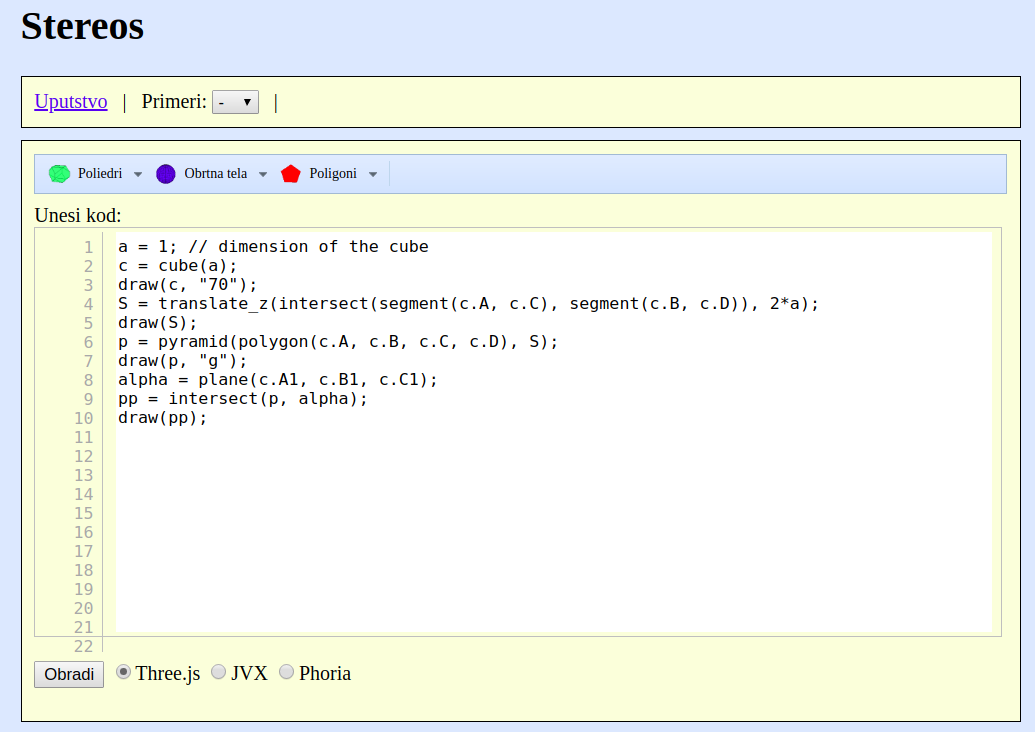
\includegraphics[height=5cm]{stereos-interface.png} \hspace{1cm} 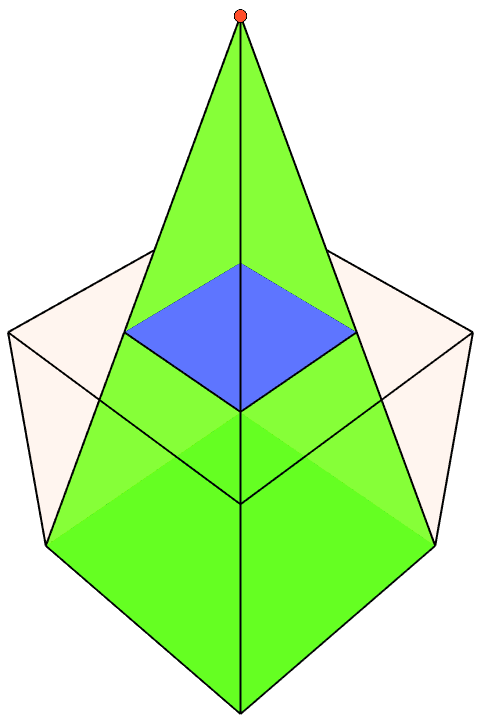
\includegraphics[height=5cm]{stereos.png}
  \caption{Stereos web interface and a produced output for Example \ref{ex:kockapiramida}}
  \label{fig:stereos}
\end{figure}

There are several important differences in the language of Stereos an
the input language of our prover described in the previous section. 
\begin{enumerate}
\item Stereos allows nested terms, while our prover language allows
  only a flat structure - each line of the input can contain only one
  relation or a function (a construction step).
\item Stereos allows only functions (construction steps), and does not
  allow relations, so geometric statements cannot be specified in the
  original Stereos language.
\item Stereos supports a richer set of construction steps than our
  prover: it natively supports intersections of solids and the planes,
  interesections of solids, 3d convex hulls, etc.
\end{enumerate}

We have made first steps towards integration of our prover and
Stereos. First, we have extended the Stereos language by adding the
command \texttt{prove} that accepts a relation over the previously
constructed objects. At this point only basic relation directly
supported by our prover can be used (for example,
\texttt{prove(orthogonal\_lines(p, q))} reduces to
\texttt{orthogonal\_lines} $p$ $q$ and \texttt{prove(A = B)} reduces
to \texttt{equal\_points} $A$ $B$. Stereos specification extended with
the \texttt{prove} statement is then converted to the input format of
our prover. Nested terms are flattened and a fresh name for each
subterm is introduced. Currently, only Stereos constructions that are
directly supported by our prover can be translated, while for all
other constructions, an \texttt{out of scope} error is reported.

Currently, Stereos is used only as a thin layer over our basic prover
so that before proving illustrations can be automatically produced
from the specification. In the future we are planning to make this
integration much tighter, and to align two different input formats so
that our prover can natively support Stereos specifications and
support more advanced construction steps that Stereos currently
supports.

\section{Conclusion and future work}

In this paper we focused on developing fully automated theorem provers
for 3d, solid geometry.

We studied two different algebraization methods for geometry
statements. The first approach introduces only coordinates of the
points involved in the construction, whereas the second approach
introduces coordinates of the objects involved in the geometry
statements such as lines, planes and objects. By comparing these two
approaches on the same set of problems, we concluded that algebraic
provers are more efficient if their input is obtained using second
approach. While testing, we noticed that the significant property is
the complexity of the polynomials in the set. The simpler polynomials
leads to better efficiency. It is especially important (if possible)
to avoid quadratic polynomials --- better approach is to substitute
complex quadratic polynomial with two or more simpler ones. Though the
smaller number of polynomials and the smaller number of variables also
help in better productivity, these two properties are not the key ones
and their impact is less obvious. Using second approach, obtained
polynomials are less complex and that is the reason why the second
approach was more convenient for algebraic provers. This suggest that
introducing line and plane coefficients as additional variables might
lead to simpler constraints and more efficient proving --- we assume
that this might also be the case in plane geometry and plan to
investigate this issue in our further work.

We implemented a prover based on the two described approaches relying
on three different third-party algebraic engines (GeoProver,
Mathematica and Maple). We also made important steps towards full
integration of our prover with the existing dynamic geometry system
Stereos. There are descriptions of applying algebraic theorem provers
on solid geometry problems \cite{shao2016challenging}, but we are not
aware of other implementations of fully automated theorem provers for
solid geometry.

During this research, we also compared different algebraic prover
engines. GeoProver's Wu's method required to be possible to transform
polynomials in the premises into triangular system. However, this
property is hard to secure and special care should be taken for
intersection of two lines. Thus, we felt more comfortable using the
other two provers, Maple's Wu's method and Mathematica's Gr\"oebner
basis method.

In our further research we plan to make thorough experiments of the
effect of the tool that we have developed in high-school and
university education. We feel that the support for automated theorem
proving in 3d geometry might have much higher impact than in 2d, since
it is much harder to observe exact relations between the geometric
objects only by looking at diagrams that are shown projected on the
two-dimensional screen. Therefore, we hope that methods and tools
described in this paper might find their way to the classrooms and
might help students.



\bibliographystyle{elsarticle-harv}
% Include the ".bib" file (generated by bibtex) right here.
\bibliography{algmethods3d}

\end{document}
